% "{'classe':('PSI'),'chapitre':'slci_correcteurs','type':('td'),'titre':'Vanoise Express', 'source':'E3A - PSI - 2014','comp':('C1-02','C2-04'),'corrige':True}"
%\setchapterimage{bandeau}
\chapter*{TD \arabic{cptTD} \\ 
Vanoise Express -- 
\ifprof Corrigé \else Sujet \fi}
\addcontentsline{toc}{section}{TD \arabic{cptTD} :
Vanoise Express -- 
\ifprof Corrigé \else Sujet \fi}

\iflivret \stepcounter{cptTD} \else
\ifprof  \stepcounter{cptTD} \else \fi
\fi

\setcounter{question}{0}
\marginnote{E3A -- PSI -- 2014.}

\marginnote{\xpComp{COR}{02}\xpComp{COR}{03}\xpComp{COR}{04}}

\begin{marginfigure} %[4cm]
\centering
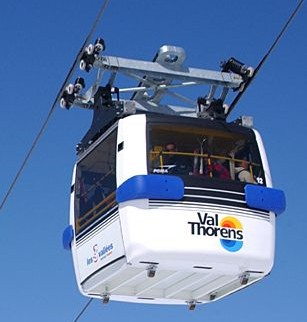
\includegraphics[width=\linewidth]{fig_00}
\end{marginfigure}






\subsection*{Présentation}

%\noindent\begin{minipage}[c]{.6\linewidth}

Le téléphérique Vanoise Express relie les domaines skiables de La Plagne et Les Arcs.% donnant naissance à paradiski, un domaine skiable de 425 km, le troisième plus grand de France.

%	Le Vanoise Express est une prouesse technologique de 16.5 millions €. C’est le plus grand téléphérique de ce type jamais construit au monde. Il est réalisé par la société POMAGALSKI. C’est un téléphérique sans pylônes, d’une seule portée de gare à gare, ce qui permet de diminuer l’impact sur l’environnement et de préserver la beauté du paysage. L’utilisation de cabines à deux étages permet de réduire le volume des cabines et des gares, améliorant l’esthétique de l’ensemble.
	
%	La solution retenue est constituée de deux lignes parallèles portant chacune une seule cabine. Contrairement à la plupart des téléphériques, les deux lignes sont entièrement indépendantes, ce qui signifie qu’une cabine n’est pas le contrepoids de l’autre. Ainsi, en cas de problème sur une cabine, la liaison entre les deux stations n’est pas interrompue.


%\end{minipage}\hfill
%\begin{minipage}[c]{.36\linewidth}
%\begin{center}
%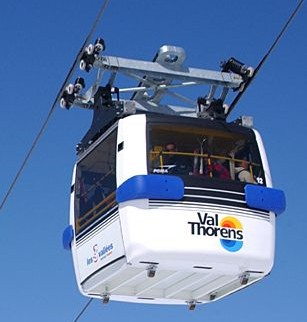
\includegraphics[width=.95\linewidth]{fig_00}
%\end{center}
%\end{minipage}

%\vspace{.25cm}
Dans ce qui suit, on désire respecter les critères suivants du cahier des charges partiel :
\begin{center}
	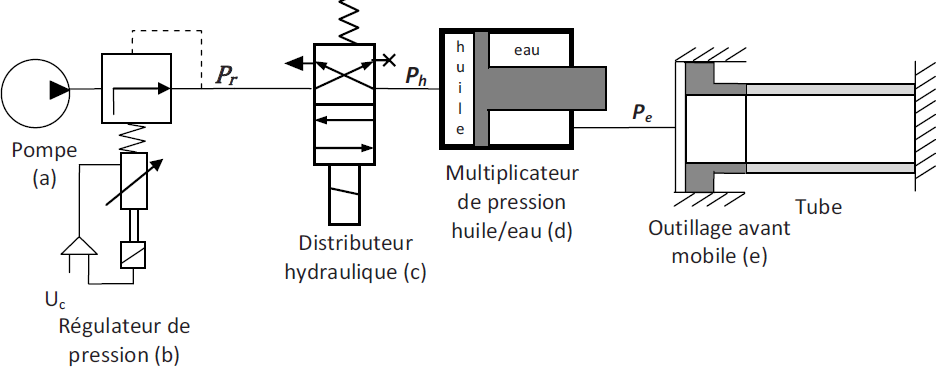
\includegraphics[width=\linewidth]{fig_01}
\end{center}

%En effet, afin de respecter les consignes de vitesse pour un trajet entre «~Les Arcs~» et «~La Plagne~», il est nécessaire que l’asservissement de vitesse des moteurs à courant continu ait des qualités en précision, stabilité et rapidité.


\subsection*{Modélisation du moteur à courant continu\sidenote{On peut passer directement à la question 6 pour aborder plus rapidement les asservissements.}}
%\begin{multicols}{2}

\marginnote{
Notations :
\begin{itemize}
\item on notera $F(p)$ la transformée de Laplace d’une fonction du temps $f(t)$;
\item $u(t)$ tension d’alimentation des moteurs;
\item $i(t)$ intensité traversant un moteur;
\item $e(t)$ force contre électromotrice d’un moteur;
\item $\omega_m(t)$ vitesse de rotation d’un moteur;
\item $c_m(t)$ couple d’un seul moteur;
\item $c_r(t)$ couple de perturbation engendré par le poids du téléphérique dans une pente et par l’action du vent, ramené sur l’axe des moteurs.
\end{itemize}}
Hypothèses et données :
\begin{itemize}
\item on suppose les conditions initiales nulles;
\item les deux moteurs sont et fonctionnent de manière parfaitement identique;
\item $L=\SI{0,59}{mH}$ inductance d’un moteur;
\item $R=\SI{0,0386}{\Omega}$ résistance interne d’un moteur;
\item $f=\SI{6}{N.m.s/rad}$ coefficient de frottement visqueux équivalent ramené sur l’axe des moteurs;
\item $J=\SI{800}{kg.m^2}$ moment d’inertie total des pièces en rotation, ramené sur l’axe des moteurs; 
\item $c_m(t)=k_Ti(t)$ avec $k_T=\SI{5.67}{Nm/A}$ (constante de couple d’un moteur);
\item $e(t)=k_E\omega_m(t)$ avec $k_T=\SI{5.77}{Vs/rad}$   (constante électrique d’un moteur)
\item équations de la dynamique : $2c_m(t)-c_r(t)=J\dfrac{\text{d}\omega_m(t)}{{\text{d}}t}+f\omega_m(t)$;
\item loi des mailles : $u(t)-e(t)=Ri(t)+L\dfrac{\text{d}i(t)}{\text{d}t}$.

\end{itemize}

%\vspace{1.7cm}


%\end{multicols}

\question{Le schéma-blocs de la double motorisation étant fourni ci-après, déterminer les fonctions de transfert $G_1(p)$, $G_2(p)$, $G_3(p)$ et $G_4(p)$ écrites dans le domaine de Laplace.}

\begin{center}
	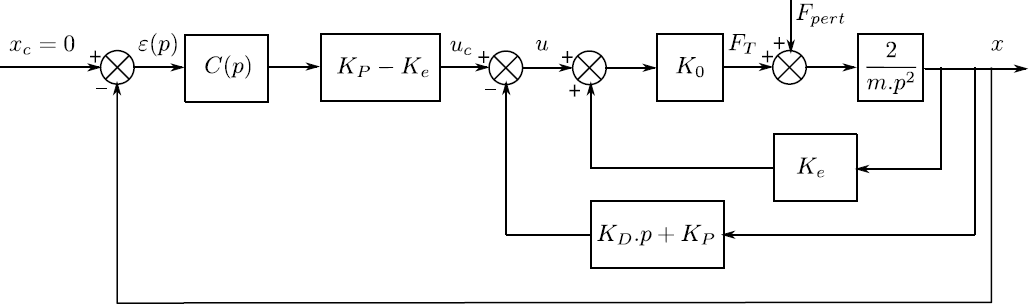
\includegraphics[width=\linewidth]{fig_02}
\end{center}

\question{$\Omega_m(p)$ peut se mettre sous la forme :  $\Omega_m(p)=F_1(p)U(p)-F_2(p)C_r(p)$. Exprimer les fonctions $F_1(p)$ et $F_2(p)$ en fonction de $G_1(p)$, $G_2(p)$, $G_3(p)$ et $G_4(p)$.}


On donne les résultats d’une simulation réalisée sur l’ensemble de la motorisation, constituée des deux moteurs à courant continu :
\begin{enumerate}
\item la première courbe représente la réponse en vitesse à un échelon de tension $u(t)$ d’amplitude \SI{100}{V} (le couple de perturbation $c_r(t)$ est nul);
\item la seconde courbe représente la réponse en vitesse à un échelon de couple de perturbation $c_r(t)$ d’amplitude \SI{1000}{N.m} (la tension $u(t)$ est nulle).
\end{enumerate}



%\noindent\begin{minipage}[c]{.48\linewidth}
\begin{marginfigure}
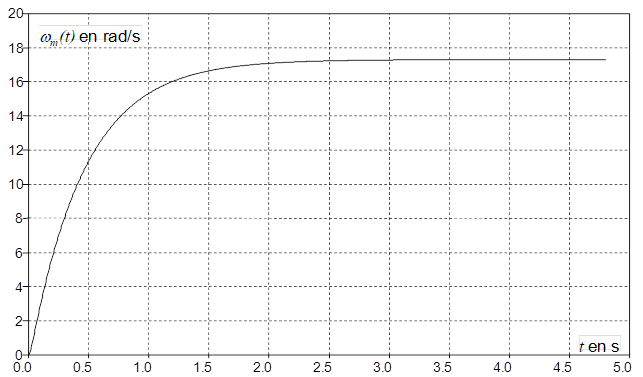
\includegraphics[width=\linewidth]{fig_06_a}

\caption{Réponse en vitesse à un échelon de tension $u(t)$ d’amplitude \SI{100}{V}.}
\end{marginfigure}

%\end{minipage}\hfill
%\begin{minipage}[c]{.48\linewidth}
\begin{marginfigure}
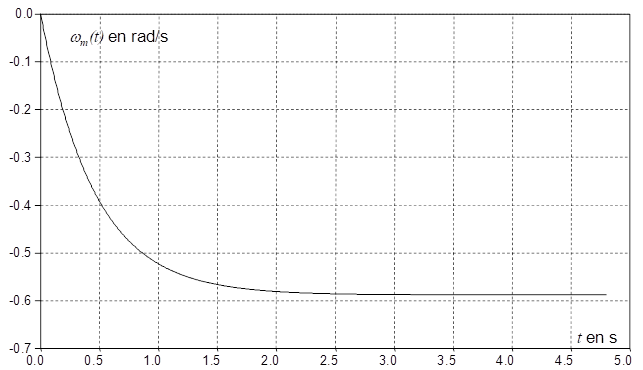
\includegraphics[width=\linewidth]{fig_06_b}

\caption{Réponse en vitesse à un échelon de couple de perturbation $c_r(t)$ d’amplitude \SI{1000}{N.m}.}
\end{marginfigure}
%\end{minipage}



\question{Choisisser et justifier un modèle d’identification de ces fonctions (premier ordre, second ordre etc...). Déterminer numériquement les deux fonctions $F_1(p)$ et $F_2(p)$ par identification.}


En faisant l’approximation que les deux fonctions $F_1(p)$ et $F_2(p)$ ont sensiblement le même dénominateur, le schéma-blocs ci-dessus peut se mettre sous la forme suivante :
\begin{center}
	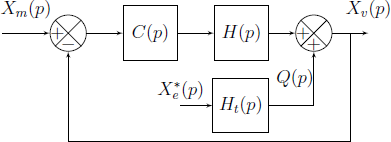
\includegraphics[width=\linewidth]{fig_03}
\end{center}


\question{Donner la valeur numérique des trois constantes $B$, $D$ et $T$.}

La motorisation modélisée ci-dessus est insérée dans une boucle d’asservissement de vitesse.

\begin{marginfigure}
	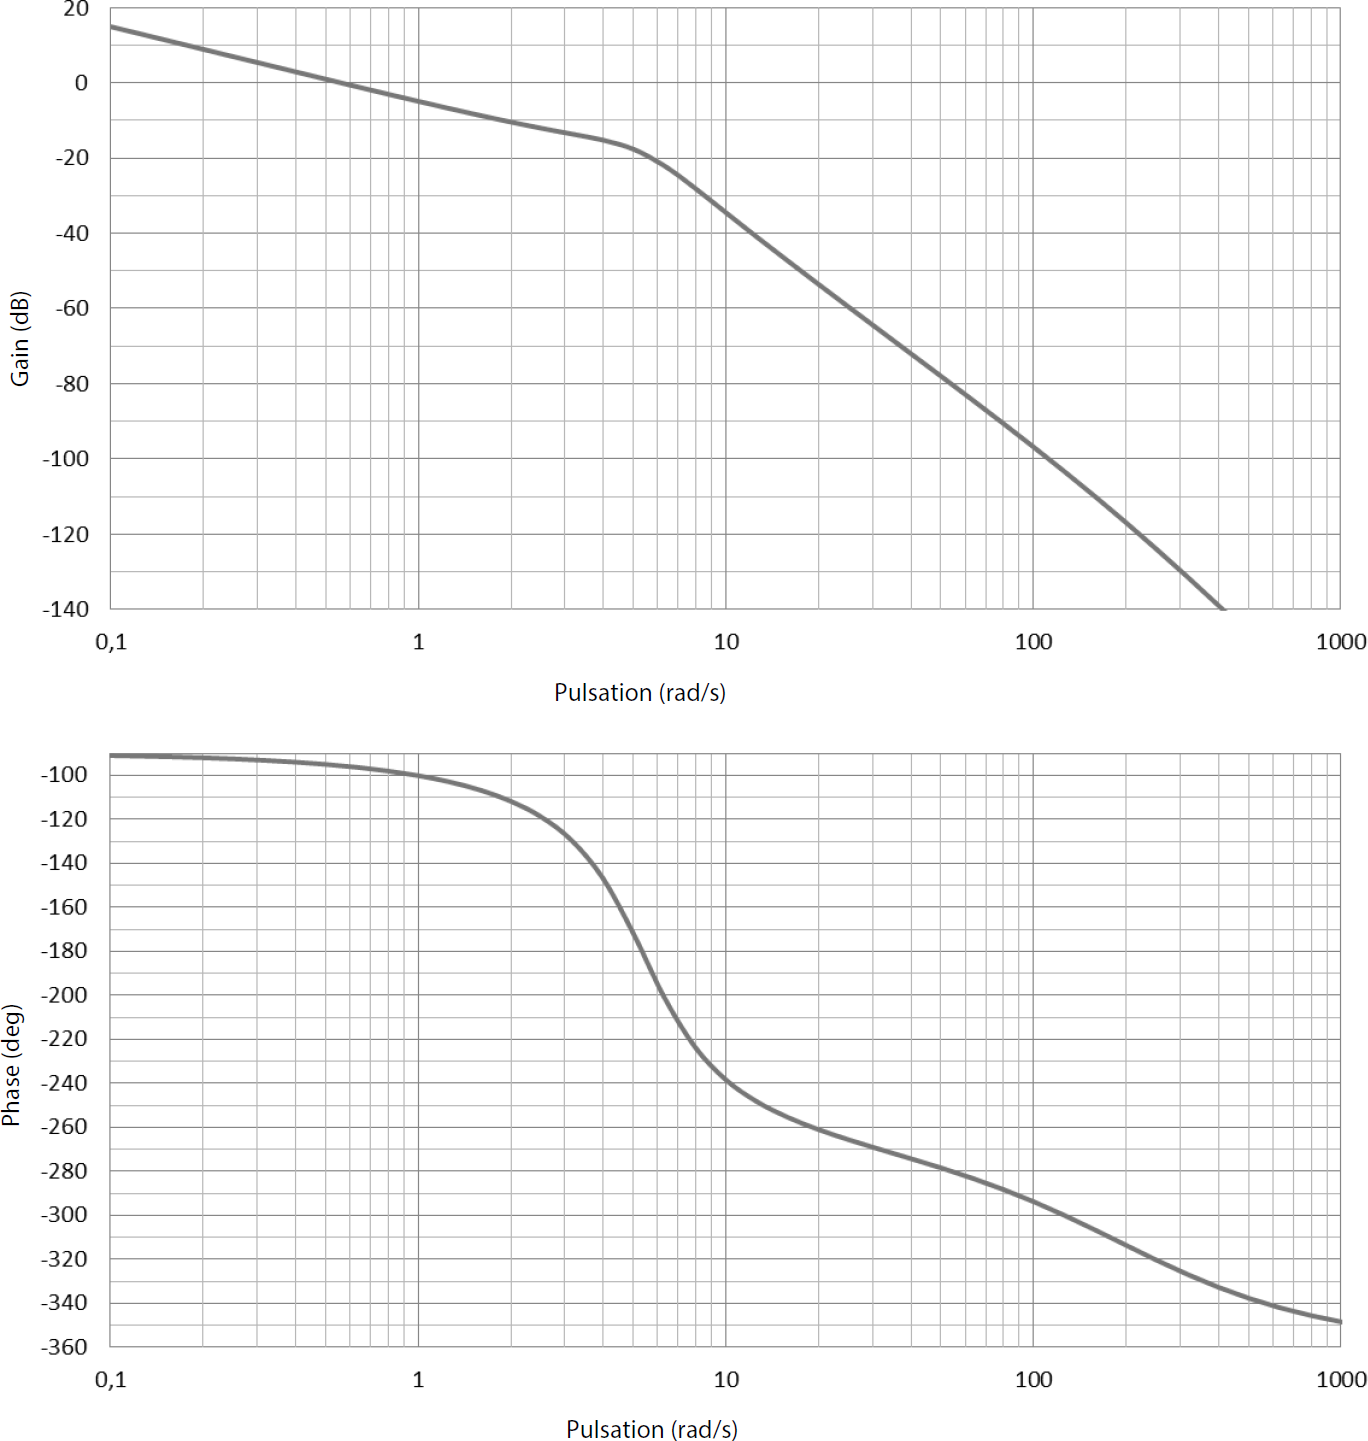
\includegraphics[width=\linewidth]{fig_04}
\end{marginfigure}

\begin{itemize}
\item La consigne de vitesse $v_c(t)$ est donnée en entrée. Elle est convertie en une tension $\rho_c(t)$ avec le gain $F$.
\item Une génératrice tachymétrique de gain $\mu=\SI{0.716}{V.s/rad}$ transforme la vitesse de rotation $\omega_m(t)$ du moteur en une tension $\rho_m(t)$.
\item Un correcteur de fonction de transfert $C(p)$ corrige la différence $\varepsilon(t)=\rho_c(t)- \rho_m(t)$ et l’envoie à un amplificateur de gain $A$, qui alimente les deux moteurs électriques.
\item La vitesse de rotation des moteurs $\omega_m(t)$ est transformée en vitesse du téléphérique $v(t)$ avec le gain $E=\SI{0,1}{m}$ (réducteur et rayon de la poulie).
\end{itemize}

%\subparagraph{}
%\textit{Déterminer l’expression du gain $E$. Faire une application numérique.}

\question{Déterminer l’expression du gain $F$ pour que $\varepsilon(t)=0$ entraîne $v_c(t)=v(t)$. Faire une application numérique.}


Par transformation du schéma-blocs, le système est mis en retour unitaire. On obtient le résultat ci-dessous :
\begin{center}
	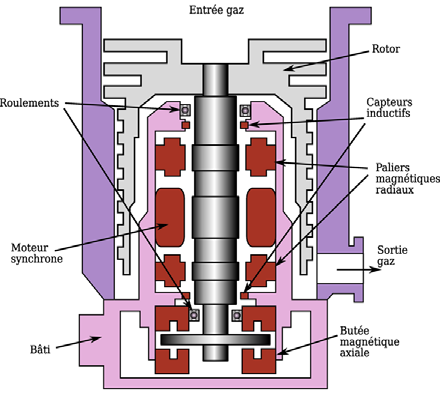
\includegraphics[width=\linewidth]{fig_05}
\end{center}

	Les coefficients $E$ et $F$ calculés précédemment sont intégrés dans les nouveaux coefficients $A’$ et $G$. Pour la suite, on continuera avec les valeurs suivantes : $A'\cdot B=3\cdot 10^{4}\;\text{sN}$; $G=6\cdot 10^{-5}\;\text{m/(sNm)}$ et $T=\SI{0,47}{s}$.
	
	
On se propose de tester successivement 3 correcteurs, et de retenir celui qui permet de respecter le cahier des charges.

\subsection*{Utilisation d'un correcteur proportionnel}
$C(p)=C_0=1$.


\question{Justifier en quelques mots que le système est stable avec ce correcteur.}

\question{On suppose $C_r(p)=0$. Calculer en fonction de $C_0$, $A’$, $B$, $G$ et $V_0$ l’expression de l’écart statique en suivi de consigne $\varepsilon'_s$ engendré par une consigne en échelon d’amplitude $V_0=\SI{12}{m/s}$. Faire l’application numérique.}



On suppose $V_c(p)=0$.
\question{Calculer en fonction de $C_0$, $A’$, $B$, $G$ et $C_{r0}$ l’expression de l’écart statique en régulation $\varepsilon''_s$ engendré par une perturbation en échelon d’amplitude $C_{r0}=\SI{-7270}{Nm}$ qui modéliserait la descente des Arcs. Faire l’application numérique.}

\question{Faire également une application numérique si $C_{r0}=\SI{7460}{Nm}$ qui modéliserait la montée vers La Plagne.}

\question{Donner numériquement l’écart statique total $\varepsilon_s=\varepsilon'_s+ \varepsilon''_s$  dans les deux cas suivants : descente des Arcs et montée vers La Plagne.}

\question{Existe-t-il une valeur réaliste de $C_0$ pour laquelle le critère «~Écart statique en vitesse en présence d’une perturbation échelon~» serait vérifié ? Justifier.}


\subsection*{Utilisation d'un correcteur intégral}

On choisit maintenant le correcteur $C(p)=\dfrac{C_i}{p}$.

\question{Donner l’expression de la fonction de transfert en boucle ouverte du système, notée $\text{FTBO}(p)$. Faire l’application numérique pour $C_i=1$.}


\question{Tracer le diagramme asymptotique de Bode de $\text{FTBO}(p)$. Tracer également l’allure des courbes. Voir figure \ref{cy:03:01:TD:02:fig:bode}}

\begin{figure}[!h]
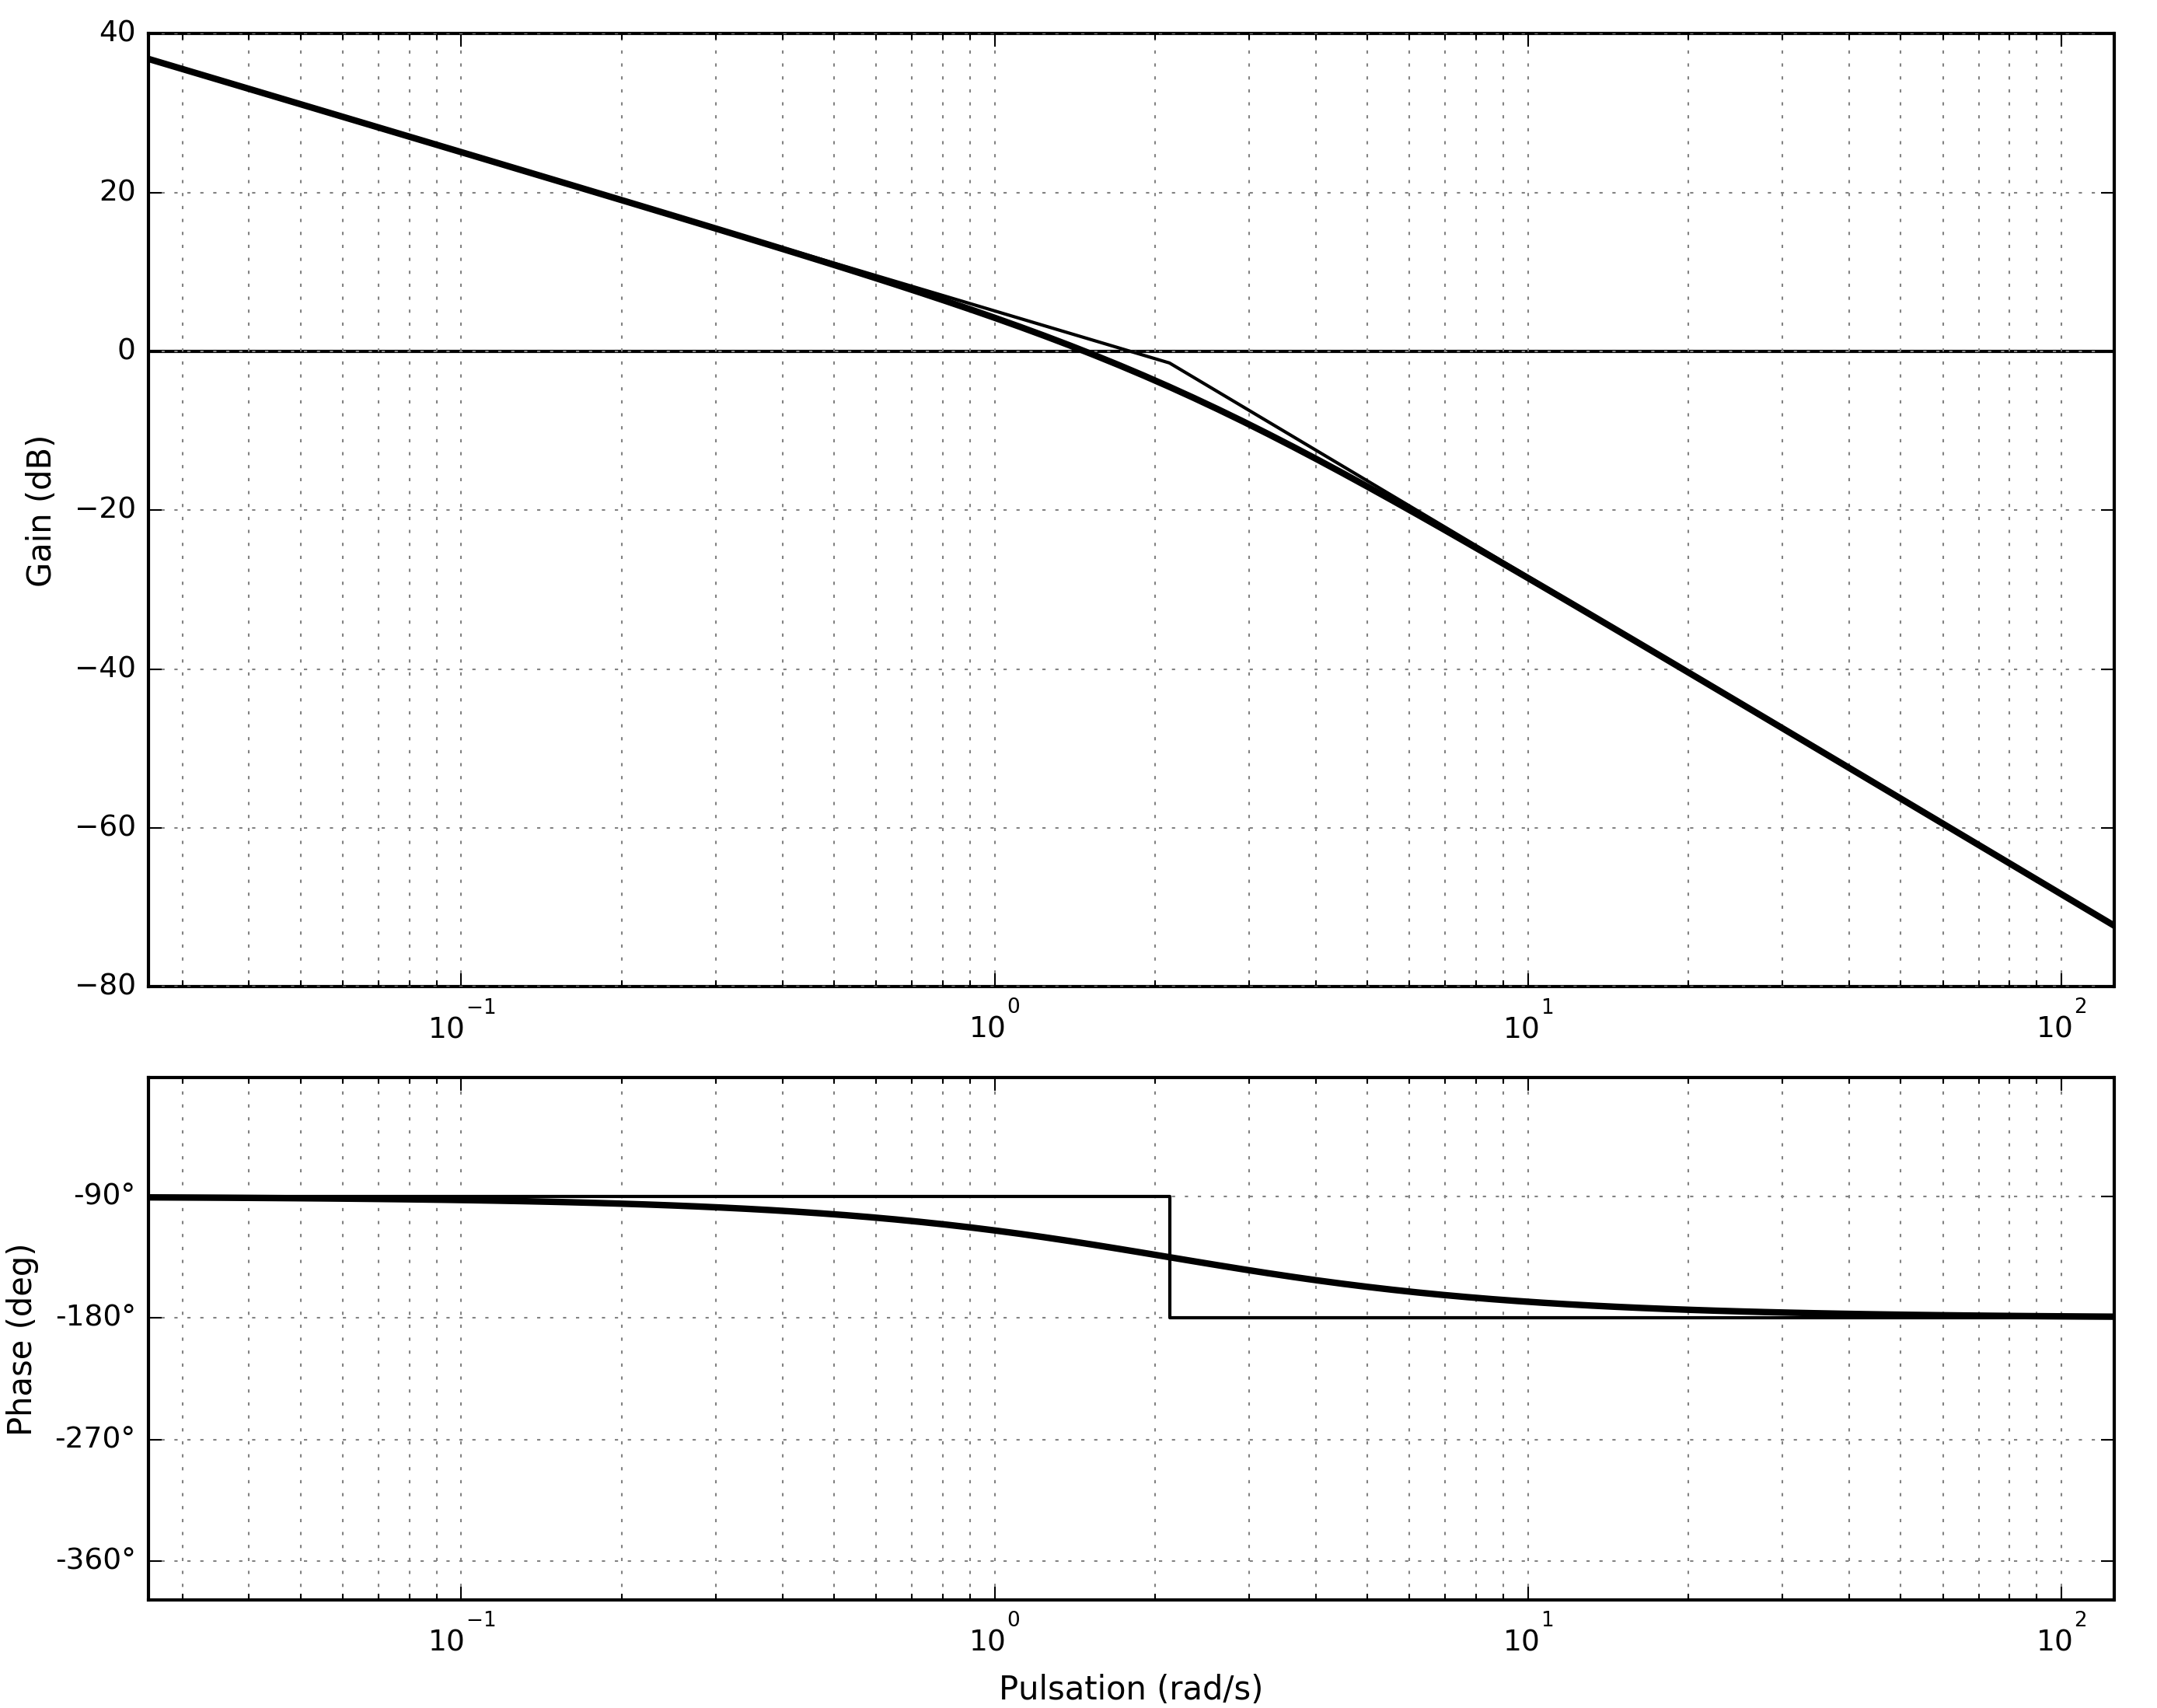
\includegraphics[width=.8\linewidth]{bode.png}
\caption{Diagramme de Bode correspondant à la question 13 ($C_i = 1$). \label{cy:03:01:TD:02:fig:bode}}
\end{figure}

\question{Donner la valeur maximale de $C_i$ permettent de respecter le critère de «~Marge de phase~» du cahier des charges ?}

\question{Trouver la valeur minmale de $C_i$ permettant de respecter le critère de «~Pulsation de coupure en boucle ouverte~» du cahier des charges ? Justifier.}
\ifprof
Il faut que la pulsation de coupure à \SI{0}{dB} soit supérieure à \SI{1}{rad/s}. Sur la BO non corrigée, on mesure que le gain vaut \SI{4,23}{dB} pour cette pulsation. On a donc $\indice{C}{i min}=0,61$.
\else
\fi
\question{On suppose Cr(p)=0. Calculer numériquement l’écart statique en suivi de consigne $\varepsilon'_s$ engendré par une consigne en échelon d’amplitude $V_0=\SI{12}{m/s}$.}

\question{On suppose $V_c(p)=0$. Calculer numériquement l’écart statique en régulation $\varepsilon''_s$ engendré par une perturbation échelon d’amplitude $C_{r0}=\SI{-7270}{N.m}$ qui modéliserait la descente des «~Arcs~».}

\question{Donner numériquement l’écart statique total $\varepsilon_s=\varepsilon'_s+ \varepsilon_s''$. Le critère «~Écart statique en vitesse en présence d’une perturbations échelon~» est-il vérifié ? Justifier.}


On suppose $C_r(p)=0$.
\question{Calculer l’expression de l’écart de traînage $\varepsilon_v$ engendré par une consigne en rampe unitaire. Existe-t-il une valeur de   réaliste qui permette de vérifier le critère «~Écart de traînage (ou écart dynamique) en vitesse en l’absence de perturbations~» ? Justifier.}

\subsection*{Utilisation d’un double correcteur intégral et d’un correcteur à avance de phase}


On décide d’utiliser le correcteur $C(p)=C_a(p)\dfrac{1}{p^2}$, produit de la fonction $C_a(p)=K\dfrac{1+a\tau p}{1+\tau p}$  avec $a>1$ (correcteur dont la fonction est d’ajouter de la phase) et d’un double intégrateur.
	On donne figure \ref{cy:03:01:TD:02:fig:07} le diagramme de Bode de la fonction $H(p)=\dfrac{A'BG}{p^2\left(1+T p\right)}$, qui est la fonction de transfert en boucle ouverte du système sans $C_a(p)$   (c’est-à-dire pour $C_a(p)=1$).

\begin{figure}[!h]
\centering
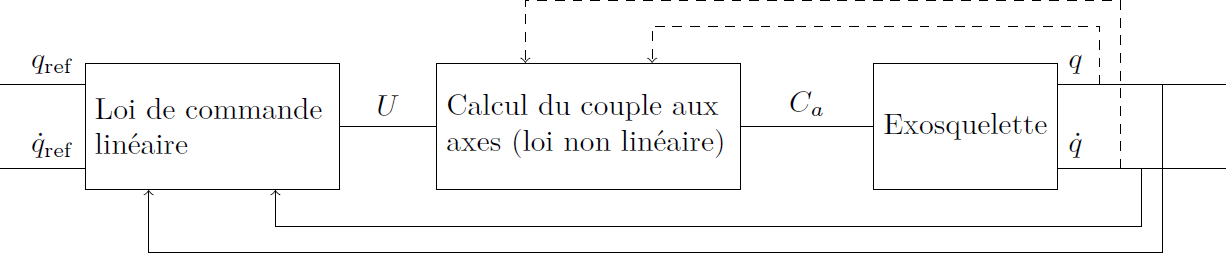
\includegraphics[width=.8\linewidth]{fig_07}
\caption{Diagramme de Bode de la fonction $H(p)=\dfrac{A'BG}{p^2\left(1+Tp\right)}$ \label{cy:03:01:TD:02:fig:07}}
\end{figure}


\question{Montrer que le système n’est pas stable sans la fonction  $C_a(p)$ ?}

	La fonction $C_a(p)$ va nous permettre de stabiliser le système et de respecter les critères de «~Marge de phase~» et de «~Pulsation de coupure en boucle ouverte~». Pour cela, il faut suivre la démarche suivante.

\question{Combien de degrés de phase faut-il ajouter à la pulsation \SI{1}{rad/s} pour obtenir une phase de $-135\degres$ ?}

\question{Tracer en fonction de $a$, $\tau$ et $K$ les diagrammes asymptotiques de Bode (amplitude et phase) du correcteur $C_a(p)=K\dfrac{1+a\tau p}{1+\tau p}$  avec a>1. Préciser clairement les amplitudes ou les phases de toutes les asymptotes horizontales en fonction des différents paramètres. Préciser de même les pulsations des points particuliers.}

\question{La phase maximum $\varphi_{\text{max}}$ ajoutée par $C_a(p)$ peut être calculée par la formule : $\sin \varphi_{\text{max}}=\dfrac{a-1}{a+1}$ . Calculer numériquement $a$ pour obtenir la remontée de phase déterminée sur le diagramme de Bode précédemment.}

Pour cette question, on pourra utiliser les propriétés de symétrie de la courbe de phase. 



\question{Donner l’expression en fonction de $a$ et $\tau$ de la pulsation $\omega$ pour laquelle la courbe de phase atteint son maximum.}

\question{En déduire la valeur numérique de $\tau$ pour que $\varphi_{\text{max}}$ soit ajoutée à la pulsation \SI{1}{rad/s}.}

\question{Calculer numériquement la valeur à donner à $K$ pour respecter les critères de «~Marge de phase~» et de «~Pulsation de coupure en boucle ouverte~» du cahier des charges ? Préciser la démarche utilisée.}

\question{Les critères «~Écart statique en vitesse en présence d’une perturbation échelon~» et  «~Écart de traînage (ou écart dynamique) en vitesse en l’absence de perturbations~» sont-ils vérifiés ? Justifier.}

\question{Ce correcteur permet-il de vérifier les critères du cahier des charges ? Justifier.}



\ifprof
\else
\begin{marginfigure}
\centering

\includegraphics[width=3cm]{Cy_03_01_TD_Synthese_02_VanoiseExp_qr}
\end{marginfigure}
\fi

\ifcolle
\else
\ifprof
\else
\begin{solution}
\begin{enumerate}
\item $G_1(p)=\dfrac{1}{R+Lp}$, $G_2(p)=k_T$, $G_3(p)=\dfrac{1}{f+Jp}$, $G_1(p)=k_E$. 
\item $F_1(p)=\dfrac{2G_1(p)G_2(p)G_3(p)}{1+2G_1(p)G_2(p)G_3(p)G_4(p)}$ et  
$F_2(p)=\dfrac{G_3(p)}{1+2G_1(p)G_2(p)G_3(p)G_4(p)}$.
\item $F_1(p)=\dfrac{0,1725}{1+0,47p}$ et $F_2(p)=\dfrac{5,8 \cdot 10^{-4}}{1+0,47p}$.
\item $B=\SI{297,4}{N.m.V^{-1}}$, $D=5,8.10^{-4}\,\text{rad.s}^{-1}\text{Nm}$ et $T=\SI{0,47}{s}$.
%\item $E=\dfrac{D}{2}k=\SI{0,1}{m}$.
\item $F=\dfrac{\mu}{E}=\SI{7,16}{V.s.m^{-1}}$
\item FTBO d'ordre 1 bouclé. Le système est stable.
\item  FTBO de classe 0 $\varepsilon_S'=\dfrac{V_0}{1+C_0A'BG}=\SI{4,286}{m.s^{-1}}$.
%\item $\varepsilon_S''=\dfrac{C_{r0}G}{1+C_0A'BG}=\SI{-0,156}{m.s^{-1}}$.
\item $\varepsilon_S''=\SI{-0,156}{m.s^{-1}}$ -- à vérifier.
\item $\varepsilon_S''=\SI{0,160}{m.s^{-1}}$.
\item $\varepsilon_S'=\SI{4,13}{m.s^{-1}}$, $\varepsilon_S'=\SI{4,46}{m.s^{-1}}$.
\item $C_0$ infini
\item $\text{FTBO}(p)=\dfrac{1,8}{p\left(1+0,47 p \right)}$
\item $\quad$
\item $\omega_{\SI{0}{dB}}\leq\SI{2,13}{rad.s^{-1}}$ et $C_i\leq1,67$.
\item $C_i\geq 0,61$.
\item FTBO de classe 1 $\varepsilon'_S=0$.
\item Intégrateur en amont de la perturbation $\varepsilon''_S=0$.
\item CDCF OK.
\item $\varepsilon_v=\dfrac{1}{C_iA'BG}$
\item Marge négative, système instable.
\item $70\degres$ de phase à ajouter.
\item $\quad$
\item $a=32,16$
\item $\omega=\dfrac{1}{\sqrt{\tau a \tau}}$
\item $\tau = \SI{0,176}{s}$
\item $K=0,109$
\item $\quad$
\item $\quad$
\end{enumerate}
\end{solution}
\fi
\fi
